% Drawing 63/05-3 -- folder 63, batch 05, archive page 99 (PDF page 100).
% Transcription: Dans la marge gauche, trois dessins : un croquis de courbes biffé par un gribouillis ; sous une accolade marquée $M'_3$, un faisceau de droites passant par le point $a$, le tout sous une accolade marquée $M_3$ ; puis, reliées par deux flèches vers le bas, une droite épaisse marquée $\mu_3^{*}$ avec le point $b$, et une droite marquée $\mathbf{Z}$ avec le point $2$.
% Kind: struck sketch; pencil of lines through a; mu_3^* over Z. Method 2 (schematic redraw from the facsimile). Status: ok.
% Notes: Middle: under a brace M'_3 on the left, a pencil of four lines through the point a (with a short vertical stroke through it), the whole under a brace M_3 on the right. Below, joined by two downward arrows: the thick line mu_3^* with the point b, and the line Z with the point 2. Omitted as struck: the first of the three drawings, at the top, a sketch of curves struck through by a scribble. Issue 128, 2026-11-09: struck material left out after a fresh check of the facsimile (struck-out material is not drawn). Redrawn 2026-11-09 (issue 128): to check again.
% Coordinates: 1 unit = 1 mm = 1/100 of the crop width (bbox in page fractions: [0.08, 0.37, 0.4, 0.57]).
% Redrawn by Claude (claude-opus-5-5), issue #73, 2026-11-07; not checked by a human; not compiled (no TeX in the session).
% Rights: reproduces part of the work -- behind RENDER_TRANSCRIPTS, never published by itself.
\documentclass[tikz,border=3pt]{standalone}
\usepackage{amsmath,amssymb}
\usetikzlibrary{patterns,arrows.meta}
\tikzset{pencil/.style={black!45}, struck/.style={black!35}, mark/.style={circle,draw,inner sep=1.3pt}, pt/.style={circle,fill,inner sep=0.9pt}, opt/.style={circle,draw,fill=white,inner sep=1.1pt}}
\begin{document}
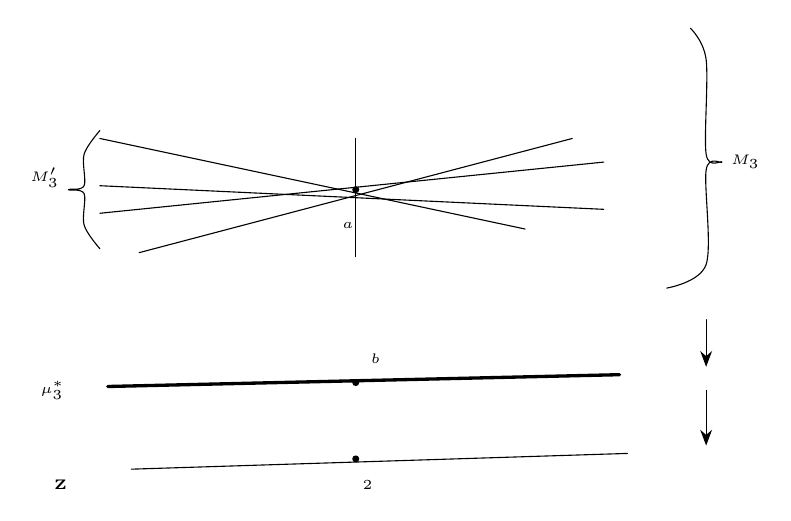
\begin{tikzpicture}[x=1mm,y=1mm,line cap=round,line join=round,font=\scriptsize]
\draw (16,-35) -- (70,-46.5);
\draw (16,-41) -- (80,-44);
\draw (16,-44.5) -- (80,-38);
\draw (21,-49.5) -- (76,-35);
\draw (48.5,-35) -- (48.5,-50);
\node[pt] at (48.5,-41.5) {};
\node[inner sep=1pt] at (47.5,-46) {\tiny $a$};
\draw plot[smooth, tension=0.55] coordinates {(16,-34) (14,-37) (14,-41) (12,-41.5) (14,-42) (14,-46) (16,-49)};
\node[inner sep=1pt] at (9,-40) {\tiny $M'_3$};
\draw plot[smooth, tension=0.55] coordinates {(91,-21) (93,-25) (93,-37) (95,-38) (93,-39) (93,-51) (88,-54)};
\node[inner sep=1pt] at (98,-38) {\tiny $M_3$};
\draw[-{Stealth[length=2mm]}] (93,-58) -- (93,-64);
\draw[-{Stealth[length=2mm]}] (93,-67) -- (93,-74);
\draw[very thick] (17,-66.5) -- (82,-65);
\node[pt] at (48.5,-66) {};
\node[inner sep=1pt] at (51,-63) {\tiny $b$};
\node[inner sep=1pt] at (10,-67) {\tiny $\mu_3^{*}$};
\draw (20,-77) -- (83,-75);
\node[pt] at (48.5,-75.7) {};
\node[inner sep=1pt] at (50,-79) {\tiny $2$};
\node[inner sep=1pt] at (11,-79) {\tiny $\mathbf{Z}$};
\end{tikzpicture}
\end{document}
